\documentclass{article}
\usepackage{epsfig}
\usepackage{amsmath}
\usepackage{amsfonts}
\usepackage{amssymb}
\usepackage{enumitem}
%\def\labexe{Expt361}

%\def\expttitle{RC and LC filters}
%\def\exptnumber{361}

%\newcommand{\IsDocumentReady}{True}
%\newcommand{\IsExperiment}{True}

%\newcommand{\expcolor}{B} % R,G,B.
%\newcommand{\ELF}{4}

%\usepackage{minted}
%\usepackage{399}
\usepackage[a4paper, total={6.5in, 9.5in}]{geometry}

\begin{document}

\title{Experiment 361}
\author{ }
\maketitle

\section*{Aim}
The responses of resistors, capacitors and inductors to (varying)
input voltages/currents can filter or amplify these input
signals. Such circuits, and their digital equivalent, are commonly
used in the electronics you use every day. This lab lets you
investigate the theoretical properties of passive RC and LC filters,
and to experimentally verify these properties.

{\bf As in all advanced lab experiments, the questions posed in this
handout merely serve as a guidance to write your comprehensive lab
report.}

\section*{Reference}
The best reference book for this lab is the stage 2 Physics 240 text
(OR IS IT 340? 244?): "Linear steady state network theory" by
G.E.J. Bold and J. B. Earnshaw. {\bf should we make this available
  somewhere?}

For more a detailed analysis of the Bode and Nyquist plots of passive
circuits try "Network analysis and synthesis" by Franklin Kuo, or any
of the many other electronics texts available in the library. {\bf Do
  we have something less than 50 years old for these students?}

\section*{Equipment list}
\begin{itemize}
\item Elvis Board with power supply and USB cable
\item Circuit components: two resistors
  $R = 10,000, 300$ and 82~$\Omega$, a conductor $L = 10$~mH, and a
  capacitor $C=22$~nF. 
\item Wires to connect the components on the Elvis Board.
\item Digital multimeter and (access to) lab RCL meter.
\end{itemize}

\section*{Introduction}
In electronics, filters are circuits which perform signal processing
functions to either remove or enhance certain frequency
components. Filters can be classified as either active or passive,
with active filters usually containing amplifying components in the
circuit and requiring an external power source. In this experiment we
shall study passive filters based on combinations of resistors,
inductors and capacitors. 

\section*{Theory}
One way to define a filter is to consider the ratio of the output to
the input. This ratio is called the transfer function. In this lab, we
will compare input and output voltages $V$, as a function of frequency
$f$. The transfer function is 
\begin{equation}
  \mathbf{T}(f)=\frac{\mathbf{V}_{out}(f)}{\mathbf{V}_{in}(f)}.
\end{equation}
% As we are dealing with AC signals in circuits containing inductors
% and resistors, the voltage transfer function will be a complex
% function containing information about both the gain and the phase
% difference between the input and output signals.
The transfer function $\mathbf{T}$ tells us how the filter responds to
a sinusoidal AC input voltage at a particular frequency $f$. Note that
the transfer function is a vector: it has a magnitude and a phase. The
\textbf{modulus} of $\mathbf{T}$ tells us the voltage gain (i.e., the
ratio of the amplitudes of the output and input voltages), and the
\textbf{argument} tells us the phase shift introduced by the filter
(i.e., the angle by which the output voltage leads the input voltage).

\subsection*{Bode plot}
The left of Figure~\ref{fig:bodenyquist} shows the Bode plot of a
filter. The bode magnitude plot displays the gain and the Bode phase
plot shows the filter's phase shift in degrees between the input and
output signals as a function of frequency. The magnitude plot is in
decibels (dB).  The transfer function can also be computed as a ratio
of input and output power, which is proportional to $V^2$. This new
transfer function is $\mathbf{T}^2$ with the unit of ``bel'' as the
power on a $log10$ scale. The more commonly used unit is one tenth of
a bel, or a decibel:
\begin{equation}
  |\mathbf{T}|_{dB}=
  10\log_{10}\left(|\mathbf{T}|^2\right) = 20\log_{10}(|\mathbf{T}|).
\end{equation}
To characterize the filtering properties of the circuit, we define the
corner or cutoff frequency as the frequency where the magntiude of the
transfer function changes by $\sqrt{2}$. This frequency is annotated
by the dashed line in the top left panel of
Figure~\ref{fig:bodenyquist}.

\begin{enumerate}
\item Show how the cutoff frequency is associated with a 3~dB change
  in gain.
\end{enumerate}

\begin{figure}
  \centering
  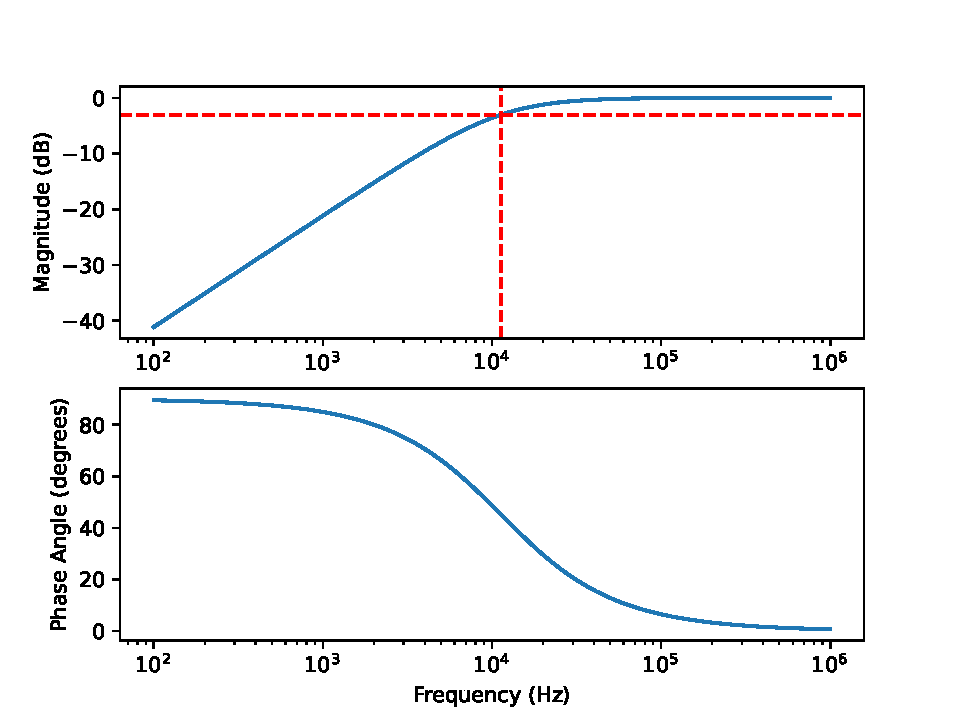
\includegraphics[width=0.49\columnwidth]{images/bodeplot} \hfill
  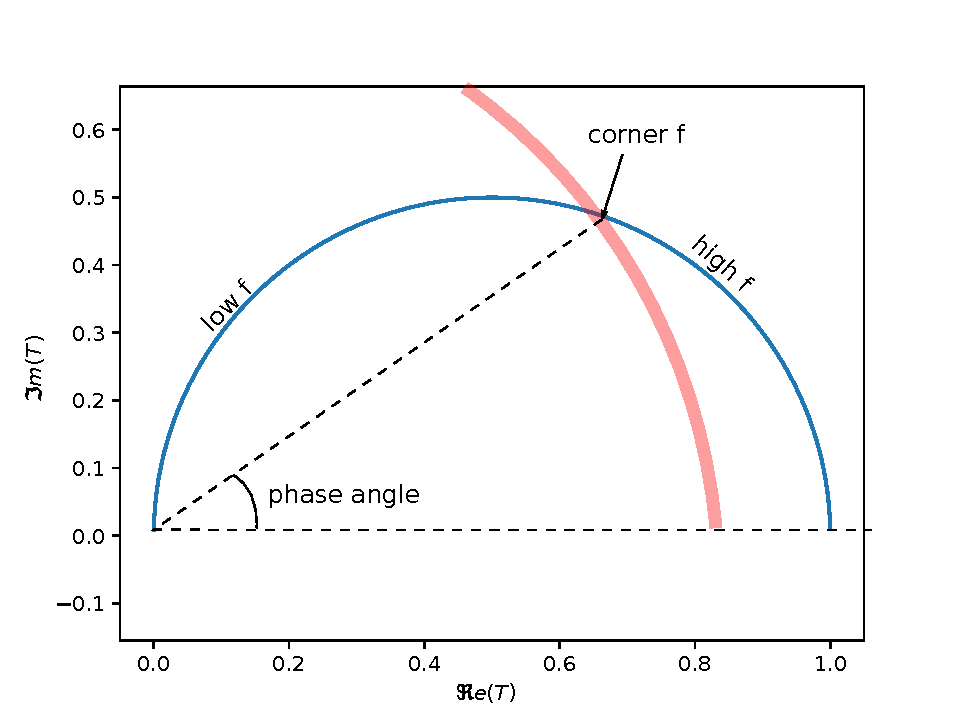
\includegraphics[width=0.49\columnwidth]{images/nyquist_annotated}
  \caption{Bode magnitude (left, top) and phase (left, bottom) plot
    for a circuit/filter with a transfer function
    $\mathbf{T}= T\exp{(i\phi)}$. The magnitude plot is
    $T=|\mathbf{T}|$, while the phase plot is $\phi$ as a
    function of frequency $f$. The corner frequency is where the
    output magnitude of the filter changes by 3~dB. Right panel: the thin
    solid line in the complex plane is the Nyquist plot. Each point on
    this line is the real and imaginary part of
    $\mathbf{T} = T(\cos(\phi)+ i \sin(\phi))$ at a particular
    frequency. The thick solid line represents the
    $|\mathbf{T}|=1/\sqrt{2}$, so the intersection of the
    solid lines represents the corner frequency. The angle is the
    phase shift of the filter at this corner frequency.}
  \label{fig:bodenyquist}
\end{figure}

\subsection*{Nyquist plot}
Because the transfer function $\mathbf{T}$ is a complex number, an
alternative way of illustrating phase and amplitude of the filter is
in one panel in the complex plane. The idea is to plot the real and
imaginary part of the transfer function $\mathbf{T}$ for a range of
frequencies, in what is called a Nyquist plot (The right panel in
Figure~\ref{fig:bodenyquist}). The length of the vector $\mathbf{T}$
represents the gain of the filter at frequency $f$, whilst the angle
of the vector with the real axis is the phase shift introduced by the
filter at that same frequency $f$.

\section*{The Elvis II+ platform}
\begin{figure}
  \centering
  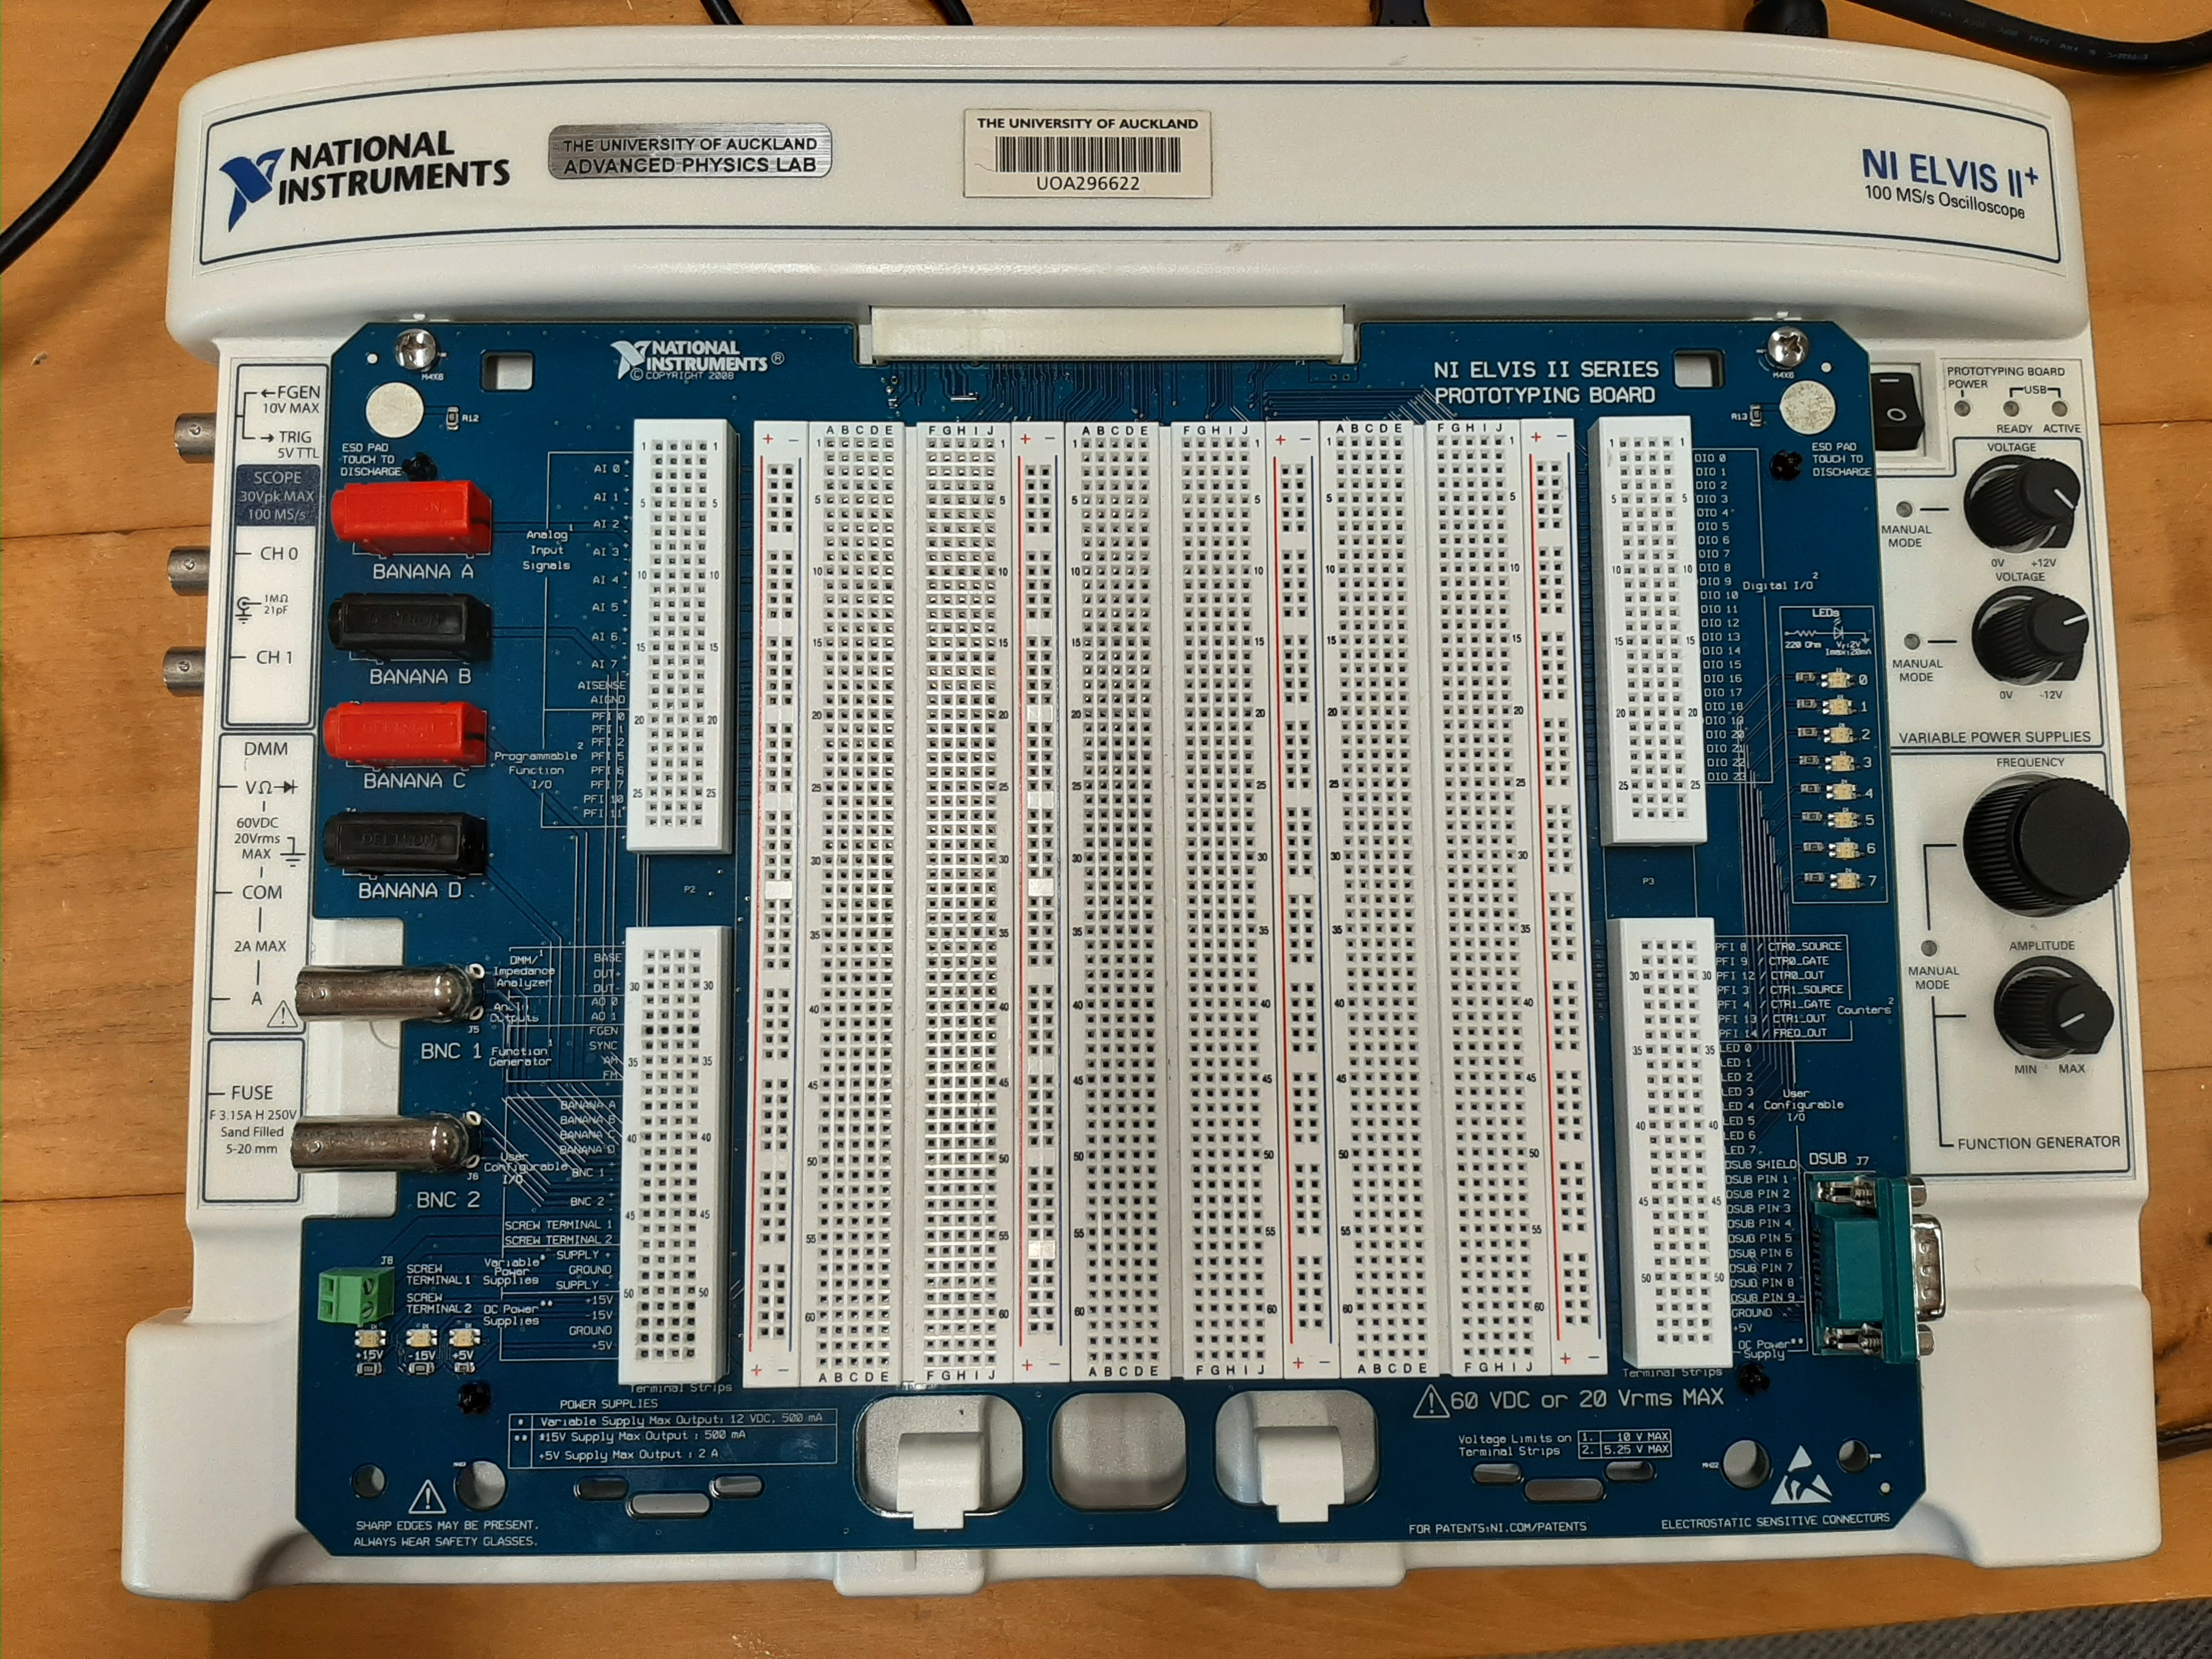
\includegraphics[width=0.5\columnwidth]{images/elvisIIplus.jpg}\\
  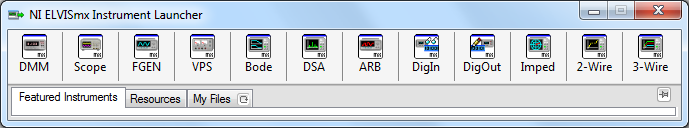
\includegraphics[width=0.5\columnwidth]{launcher.png}
  \caption{Top: the Elvis II+ board. Bottom: The
    Graphical User Interface (GUI, or ``instrument launcher''), containing
    such useful devices as the digital multimeter (DMM), an
    oscilloscope (Scope), a function generator (FGEN) and a Bode
    analyser (Bode).}
  \label{fig:elvisii}
\end{figure}
We will build electronic circuits that act as filters to an
oscillatory input voltage on a platform from National Instruments
called the ``Elvis Board'' (see the top panel of
Figure~\ref{fig:elvisii}). The breadboard of the Elvis Board allows
circuits to be tested without having to use solder to connect
components. Furthermore, the Elvis Board contains a function generator
to apply an oscillating voltage to put into your circuit, and also a
digital oscilloscope to interrogate the output of the signal that runs
through your circuit. A USB cable connects the ELVIS II+ board to a PC
with the appropriate software installed (the GUI is shown in the
bottom of Figure~\ref{fig:elvisii}), so you can control the function
generator, the oscilloscope settings, and display the outputs.  To
access these tools inside the Elvis board, ensure that the USB plug is
connected to a PC and the Elvis II+ is powered on with the switch on
the side of the device. The LED indicator for the USB should display
`READY'. You can now launch the GUI called `NI ELVISmx Instrument
Launcher.'

In this experiment we will use the Elvis' built-in function generator
to drive a circuit built on the breadboard. The Bode plot analyzer
will be used to probe the voltage across the different components of
your circuit. The Elvis board has many options to build and test a
circuit. Here, we explain one way to set up your board. This requires
three connections to be made between the Elvis and the circuit board
under test:
\begin{enumerate}[resume]
\item Activate the function generator by connecting two bare wires
  from pin 33 (FGEN on left hand plug board of ELVIS) and pin 49 (GND
  on left hand plug board of ELVIS) to the input of the circuit you
  wish to test using alligator clips.
\item Connect a BNC cable with alligator clips between oscilloscope
  channel 0 (top left hand side of the Elvis) and the input of the
  circuit you wish to test. The black lead goes to ground, and the
  lead with the other colour (blue, or red) is the positive.
\item Connect a BNC cable with alligator clips between
  oscilloscope channel 1 (top left hand side of the Elvis) and the
  output of the circuit you wish to test. The black lead goes to
  ground, the other colour is positive.
\item Launch the Bode function analyzer program from the GUI to
  measure Bode amplitude and phase plots over a frequency
  range defined in the GUI.
\item Save your data from the graphical user interface of the ELVIS
  board, under the ``log'' button. You can then import your data into
  Python to analyse and plot the results. Save these plots for your
  report. There are many ways to import the data in python, but one of
  our favourites is using the pandas package. All python packages you
  need are installed on the lab computers, or you can use Google's
  COLAB to do your computing in the Cloud.
\end{enumerate}
\section*{Experiments}
In this lab, you will explore two types of passive filters: RC and LC
filters. The former contains a circuit made of resistors (R) and
capacitors (C), while the latter is a circuit with inductor(s) L and
capacitor(s) C.

\begin{enumerate}[resume]
\item Before we build any circuits and measure the transfer function,
  consider an alternating current. What is the impedance of $R$, $C$
  and $L$? Describe these expressions in words, as well. Explain
  mathematically, but also physically, the behaviour of each component
  in the limit of very high and very low input frequencies.

  Revisit your PHYS121 book and your course notes, if you have to. %see
  % https://www.allaboutcircuits.com/textbook/alternating-current/chpt-6/q-and-bandwidth-resonant-circuit/
  % capacitor has a large impedance at low f, and low
  % impedance at high f. The inductor is opposite, and R is
  % f independent.
\end{enumerate}
  
\subsection*{RC Filters}
The simplest of filters is one with a resistor $R$ and a capacitor $C$
in series (Figure~\ref{fig:filterAB}). Such a circuit acts as a
filter, because the impedance of a capacitor is frequency
dependent. Let us explore both experimentally and theoretically the
filtering capabilities of this simple circuits.

\subsubsection*{Filter A}

{\bf Kasper, maybe switch A and B? Then you can talk about the
  impedance of a capacitor, decreasing with f?}

Filter A is the output measured over the resistor $R= 10~k\Omega$.
\begin{enumerate}[resume]
\item build the circuit of Figure~\ref{fig:filterAB} with a resistor
  $R=10~k\Omega$ and a capacitor $C=22$~nF on your Elvis board.
\item Set the function generator on your Elvis board to sweep the
  input voltage from 100 Hz to 1MHz. {\bf Set the number of samples high!} 
\item Measure the ratio of the voltage across the resistor $R$ over
  the input voltage with the Bode Analyser on your Elvis Board. What
  is this ratio called?
\item Save your data and plot these in python as a phase and
  magnitude Bode plot.
\item Explain in your report why the voltage drop across the resistor
  in the circuit of Figure~\ref{fig:filterAB} is a fraction of the
  input voltage:
  $$\mathbf{V}_{out}(\omega)=
  \frac{R}{R+{\frac {1}{j\omega C}}}\mathbf{V}_{in}(\omega).$$
  % Apply Kirchhof's Law: the voltage drop over the two components
  % needs to add to the input voltage.
\end{enumerate}
\begin{figure}
  \centering
  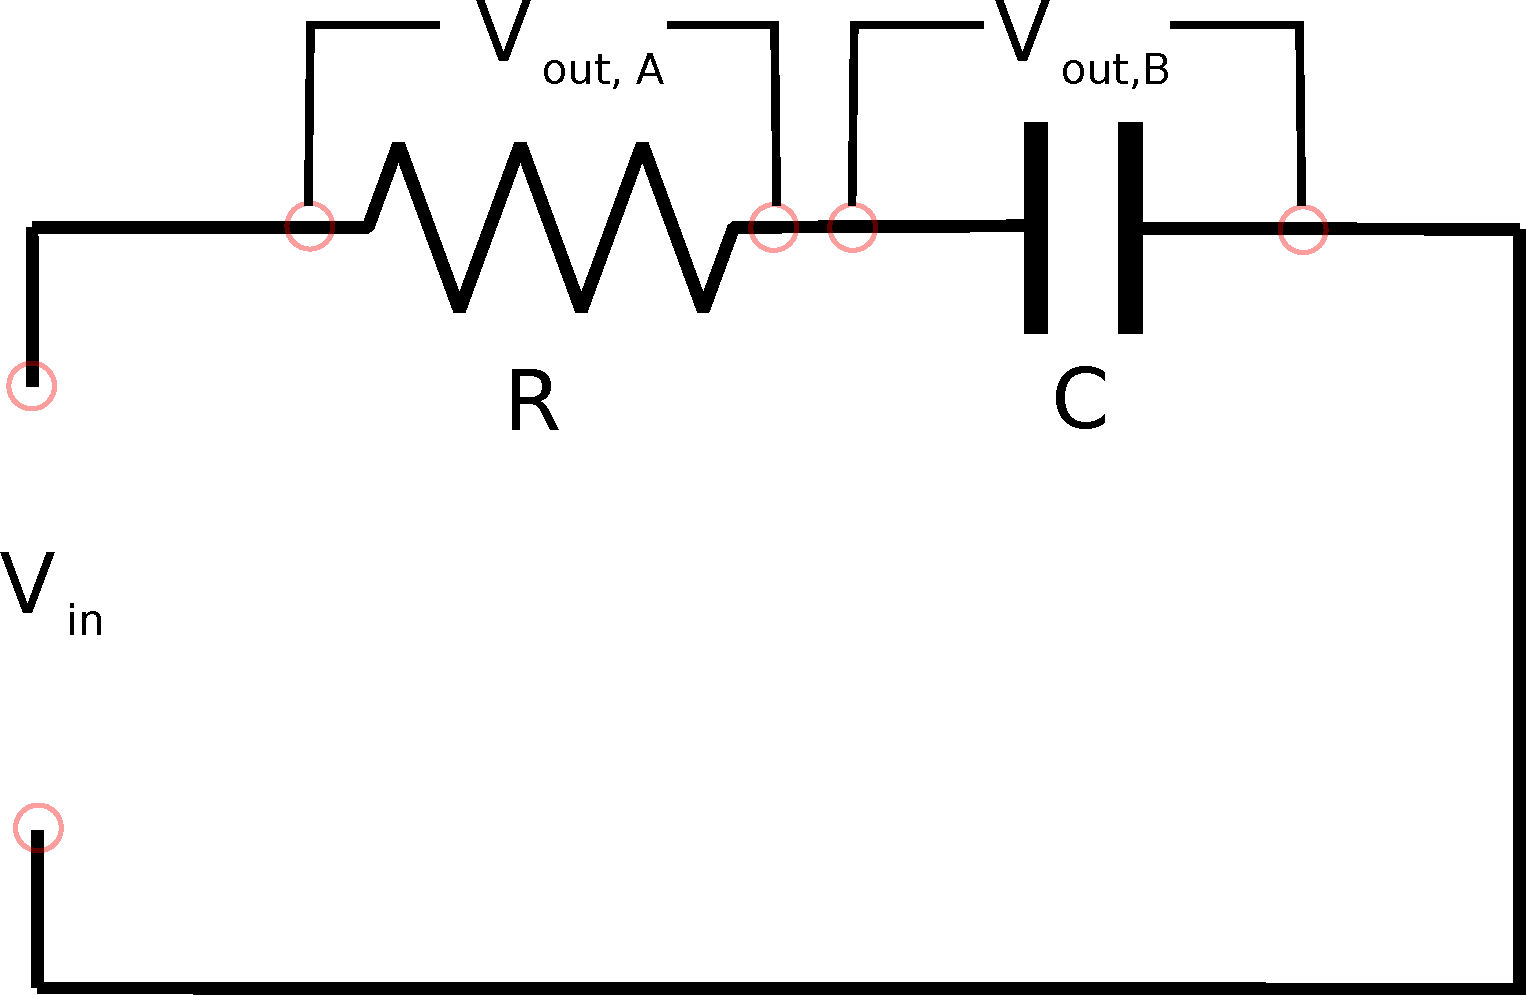
\includegraphics[width=0.5\columnwidth]{images/RCfilter}
  \caption{Circuit diagram of filters A and B. The input is $V_{in}$,
    and the outputs are $V_{out,A}$ for filter A, and $V_{out,B}$ for
    filter B.}
  \label{fig:filterAB}
\end{figure}

In PHYS121 you learned that the impedance of the capacitor is
$Z_c= 1/(j\omega C),$ where $j$ is the imaginary unit, and
$\omega = 2\pi f$ is the angular frequency. The transfer function of
Filter A is then
\begin{equation}
  \mathbf{T}_A=\frac{\mathbf{V}_{out, A}}{\mathbf{V}_{in}}=
  \frac{R}{R+1/(\mathrm{j}\omega C)}=\frac{1}{1-\mathrm{j}\omega_0/\omega},
\end{equation}
where
\begin{equation}
  \omega_0=\frac{1}{RC}.
\end{equation}
\begin{enumerate}[resume]
\item Based on what you read so far in this hand-out, show that
  $\omega_0 = 1/RC$ is the cutoff, or corner, angular
  frequency. % if $\omega = \omega_0$, then $T_A = 1/\sqrt{2}$.
\item What is $\omega_0$ for Filter~A?
\item Use Python to plot a theoretical Bode amplitude plot (in
  dB) and Bode phase plot (in degrees) on the same figure, using a
  frequency range of 100Hz-1MHz.
\item On a separate figure, use Python to
  construct a theoretical Nyquist plot from your data.
\item Explain why the output voltage measured
  across the resistor is almost zero for very low
  frequencies. 
\item What sort of output waveform ($\mathbf{V}_{out}$) would you
  expect to see on an oscilloscope from this filter when using a 1kHz
  square wave as your input waveform
  ($\mathbf{V}_{in}$)? % The flat parts of the square wave are DC-like
  % and filtered to zero. Only the sharp changes
  % contain high f and remain, leaving a saw-tooth
  % pattern.
\end{enumerate}

Filter A, as shown in Figure~\ref{fig:filterAB}, is a simple high-pass
phase-advance filter, commonly used for inter-stage coupling where DC
isolation is required.  High pass filters are characterised by their
ability to allow high frequencies to pass through the filter while
suppressing low frequencies.

\subsubsection*{Filter B}
Filter B is the output measured over the capacitor in the same
circuit ($\mathbf{V}_{out, B}$ in Figure~\ref{fig:filterAB}).

\begin{enumerate}[resume]
\item Show that this output is
  \begin{equation}
    \mathbf{V}_{out, B}=
    {\frac {1}{1+j\omega/\omega_0}}\mathbf{V}_{in}.
  \end{equation}
  %%% Now the input to output voltage ratio is over the capacitor!
  
\item Show that the transfer function for Filter B is then
\begin{equation}
  \mathbf{T}_B =
  \frac{1}{1+j\omega/\omega_0}.
\end{equation}
\item Make Bode plots of the theoretical and experimental transfer
  function $\mathbf{T}_B$.
\item What is $\omega_0$ for Filter B? 
\end{enumerate}
Based on your measurements and theoretical calculations, Filter B in
the circuit in Figure~\ref{fig:filterAB} is a simple low-pass
phase-delay filter used to remove unwanted high-frequency signals.

\subsubsection*{The relationship between Filters A and B}
Because the circuit used for Filters A and B is the same, the output
for Filter B can also be derived from the output of Filter A, because
Kirchhoff's Law says
\begin{equation}
  \mathbf{V}_{in}=\mathbf{V}_C+\mathbf{V}_R
\end{equation}
Therefore,
\begin{equation}
  \mathbf{T}_B =\frac{\mathbf{V}_C}{\mathbf{V}_{in}}
  =\frac{\mathbf{V}_{in}-\mathbf{V}_R}{\mathbf{V}_{in}}
  =1-\frac{\mathbf{V}_R}{\mathbf{V}_{in}}
  =1-\mathbf{T}_A.
\end{equation}

\begin{enumerate}[resume]
\item Plot Filters A and B together in one panel for a Bode amplitude
  plot, and one for a Bode phase plot.
\item As the voltage transfer function $\mathbf{T}_B$ can be derived
  from the voltage transfer function for Filter A, construct a Nyquist
  plot by by adding $-\mathbf{T}_A$ to $\mathbf{1}$ vectorially. This
  vector addition is equivalent to addition of complex numbers.
\item Discuss how the Bode and Nyquist plots inform us about the relations
  between these two filters.
\end{enumerate}

\section*{LC filters}
\begin{figure}
  \centering
  \includegraphics[width=0.45\columnwidth]{images/LCseries} \hfill
  \includegraphics[width=0.45\columnwidth]{images/LCparallel}
  \caption{Circuit diagram for Filter C (left) and Filter D
    (right).}
  \label{fig:filterCD}
\end{figure}
We just saw that RC filters act as high- or low-pass filters. If we
replace the resistor $R$ with a inductor $L$, we have an LC circuit.
We will see that LC filters are able to act as an electrical
resonator. These resonant properties can be used to select certain
frequencies out of a range of frequencies, making them useful for
applications such as tuning radio transmitters and receivers, but also
the scientific equipment we use in Physics.

For the LC filters, let us replace the load of $R=10~k\Omega$ with a
smaller one: $R= 300~\Omega$ on the Elvis Board and for your
simulations.

\subsection*{Filter C}
The left panel of Figure~\ref{fig:filterCD} is the circuit, where the
voltage output over resistance $R$ is Filter C.  $R_s$ represents the
resistance of the inductor-capacitor series combination. There does
not need to be a physical resistor there, but any inductor-capacitor
in series will create a resistance of the inductor and capacitor. This
resistance transfers electric energy to heat, causing electrical power
loss.

\begin{enumerate}[resume]
\item Use the Elvis board to obtain an experimental Bode plot for
  Filter~C.
\end{enumerate}

The voltage transfer function of Filter C is
\begin{equation}
  \mathbf{T}_C=\frac{\mathbf{V}_{out}}{\mathbf{V}_{in}}=\frac{R}{R+z_s},
  \label{eq:D1}
\end{equation}
where the impedance of the inductor and capacitor in series is
\begin{equation}
  z_s=Z_{R_S}+ Z_C + Z_L = R_s+j\left(\omega L-\frac{1}{\omega  C}\right)
  \label{eq:D2}
\end{equation}
From equation \ref{eq:D1}, we can see that $|\mathbf{T}_C|$ is a maximum
when $|z_s|$ is a minimum.
\begin{enumerate}[resume]
\item Derive from equation~\ref{eq:D2} that this maximum occurs when
  $\omega=1/\sqrt{LC}$.  This angular frequency when the response of
  the filter is a maximum is called the resonant frequency
  $\omega_0 = 1/\sqrt{LC}$. % set the derivative to zero
\item In Python create Bode magnitude plots of Filter C with the
  values of $R,C$ and $L$ of your circuit. Vary $R_S$ until you match your
  observed transfer function. You may have to refine the true values
  of $R$, $L$ and $C$, too!
\end{enumerate}
Hopefully, your plots illustrate that the smaller the internal resistance
$R_s$, the sharper the peak of the transfer function in the Bode
amplitude plot. As we said before, $R_s$ converts electrical energy to
heat. A parameter to measure the energy lost per cycle (i.e.,
oscillation) is the quality factor
\begin{equation}
  Q = \times {\frac {\text{maximum energy stored}}{\text{power loss per cycle}}}
\end{equation}
A practical result of this definition is that {REFERENCE WITH
  DERIVATION}:
\begin{equation}
  Q =  \frac {f_0}{\Delta f}=\frac {\omega _0}{\Delta \omega },
  \label{eq:Q}
\end{equation}
where $f_0$ is the resonant frequency, $\Delta f$ is the resonance
width or Full Width at Half Maximum (FWHM). This is the {\bf
  bandwidth} over which the power is greater than half the power at
the resonant frequency. Therefore, a filter with a large bandwidth has
a low $Q$, and vice versa.

\begin{enumerate}[resume]
\item What is ``half power'' in dB?
\item Estimate the quality factor of filter $Q_C$ from the Bode plot
  of your exierimental data for this filter.
\end{enumerate}

We already saw that $Q_C$ is inversely proportional to $R_s$. In
more advanced electronics courses and books (REFERENCE!) you may
derive the full relationship:
\begin{equation}
  Q_C=\frac{\omega_0 L}{R + R_s}.
  \label{eq:Qc}
\end{equation}
\begin{enumerate}[resume]
\item Even though we do not derive the equation, discuss how the
  resistance(s) in Filter C affect $Q_C$.
\item Compare $Q_C$ with equation~\ref{eq:Qc} and the information you
  obtained about the values of the electronic components to your
  estimate of $Q_C$ from equation~\ref{eq:Q}.
\end{enumerate}

The concept of the quality factor is not only used in electronics, but
also in laser physics to describe the energy loss in an optical
cavity, in mechanical engineering, and in seismology to study the
normal modes of vibration of the Earth.

\begin{enumerate}[resume]
  
\item Maybe keep this as an oral exam question: describe the filtering
  powers of this circuit when $V_{out}$ is measured over the RLC
  combo. Could be used for Filter D too, of course.
  % many ways to show that this is the inverse of Filter C: a notch
  % filter at omega_0. Could use equation for zs, or use Kirchhoff's
  % Law + a Nyquist plot. This will show if the student understood the
  % Filter A/B connection.
\end{enumerate}

\subsection*{Filter D}
Filter D The circuit shown on the right in
Figure~\ref{fig:filterCD}. It shows an LC circuit, with the
resistance $R_p$ representing the resistance from the inductor and
capacitor in parallel. The voltage transfer function for this circuit
is given by:
\begin{equation}
  \mathbf{T}_D=\frac{\mathbf{V}_{out}}{\mathbf{V}_{in}}=\frac{R}{R+z_p},
\end{equation}
where the impedance of the parallel components is 
\begin{equation}
  z_p\equiv \frac{1}{1/Z_{R_P}+1/Z_C+1/Z_L}=
  \frac{R_p}{1+\mathrm{j}R_p\left(\omega C - \frac{1}{\omega L}\right)},
\end{equation}
where the resistance $R_p$ is the parallel loss resistance
of the inductor (the capacitor has negligible loss resistance).
\begin{enumerate}[resume]
\item Explain as you did in Filter C what you expect the filtering
  behaviour to be for Filter D.
  % $|z_p|$ is a
  % maximum at the resonant
  % frequency, %where $\omega=\omega_0=1/\sqrt{LC}$, i.e.\ at the frequency
  % $\omega_0=1/\sqrt{LC}$. This makes Filter D a notch filter, or
  % band-reject. Check this.
  
  %We can define $Q_p$ as the Q factor of the parallel inductor-capacitor
  %combination, which gives a measure of how damped the system is. $Q_p$
  %is given by {\bf big step 1:}
  %\begin{equation}
  %  Q_p=\frac{R_p}{\omega_0 L}=\omega_0 R_p C.
  %\end{equation}
  %The Q factor of Filter~D (different from $Q_p$) can then be defined as
  %{\bf Because? Step 2 (I cannot get there, yet):}
  %\begin{equation}
  %  Q_D=Q_p\sqrt{1-2|\mathbf{T}_{D}|_{min}^2},
  %\end{equation}
  %where $|\mathbf{T_D}|_{min}$ is the minimum value of $|\mathbf{T}_D|$.
  
\item Use the Elvis board to obtain a Bode plot for this filter.
\item Estimate the value of $R_p$, the way you did
  for Filter C: by fitting your data to the theoretical Bode plot.
  
\item Estimate the quality factor for Filter D using your measurements
  and equation~\ref{eq:Q}
\item Maybe not surprisingly, $Q_D = \frac{R_p+R}{\omega_0
    L}$. Compare this to $Q_C$ and note the symmetry in going from a
  series to a parallel LC circuit. We do not derive this, but you can
  check if you get the same or similar value for $Q_D$ as from your
  experimental Bode plot.
\item Question I do not know the answer to: Should $R_p$ and $R_s$ be
  the same?
\item Question for our colleagues: should we derive $Q_c$ and $Q_d$? Does
  that make the lab too long or too theoretical?
\end{enumerate}


%{\bf Left out the bit about critical damping etc. Not sure how much it
%  adds here, in the f-domain? A cool lab would show electrical,
%  optical and mechanical resonances, investigating the similarities
%  and differences. Critical damping is ``critical'' in damping a
%  seismograph.}

S. Ruddell, S. Murdoch February 2013

S. Coen 2021

K. van Wijk, 2022
\end{document}


